In this chapter I will describe obtained results on each test machine. I will show scheduling executed by task-affinity and effects on cache miss and 
task migration. 

In Fig. TODO they are represented the ideally scheduling that the developed patch and vanilla should perform. I have said "ideally" because, as described 
in \cite{lcs}, it is impossible to perform this scheduling, because scheduling latency are not equal for each core.
 
TODO fig schedule

In the picture, time is normalized to the duration of one sample, in this way, it is possible express duration of different tasks in relative terms.
According to experiment performed, on Intel xeon \textit{waves} represent $~40\%$ of the sample, \textit{mixer0} and \textit{mixer1} represent $~60\%$.
On Intel i7 

As we can see, the scheduling proposed, should significantly improve throughput. To estimate this improvement we use the \textit{amdhal's law} \cite{lcs}:

\begin{equation}
       Speedup = (\frac{P_{1}}{S_{1}} + \frac{P_{2}}{S_{2}} + ... \frac{P_{n}}{S_{n}})^{-1} 
\label{eq:amdhal}
\end{equation}

Where $P_{i}$ is the i-th parallelized portion of the program and $S_{i}$ is the correspondent speedup. Furthermore the following constraint must be 
respected

\begin{equation}
       sum_{i=1}^N P_{i} = 1
\label{eq:contr_amdhal}
\end{equation}




In the proposed scheduling \textit{mixer2} is executed in parallel with waves, therefore during the execution of \textit{waves} and \textit{mixer2} 
theorical speedup should be \textit{x5}, while in the scheduling performed by vanilla, during the execution of \textit{waves} speedup is $x4$ and during
the execution of  \textit{mixer2} there is any speedup, because \textit{mixer2} is executed alone.

TODO dirci qualcosa


In this chapter I will show the behaviour of task-affinity on different architectures. First of all, using \textit{trace}, we will check if expected 
scheduling is performed, after which we will analyze how optimization proposed influence performance and L1 and LLC miss rate of the application. 

%%%%%%%%%%%%%%%%%%%%%%%%%%%%%%%%%%%%%%%%%%%%%%%%%%%%%%%%%%%%%%%%%%%%%%%%%%%%%
\section{Intel Xeon}

\begin{figure}[htbp]
\centering
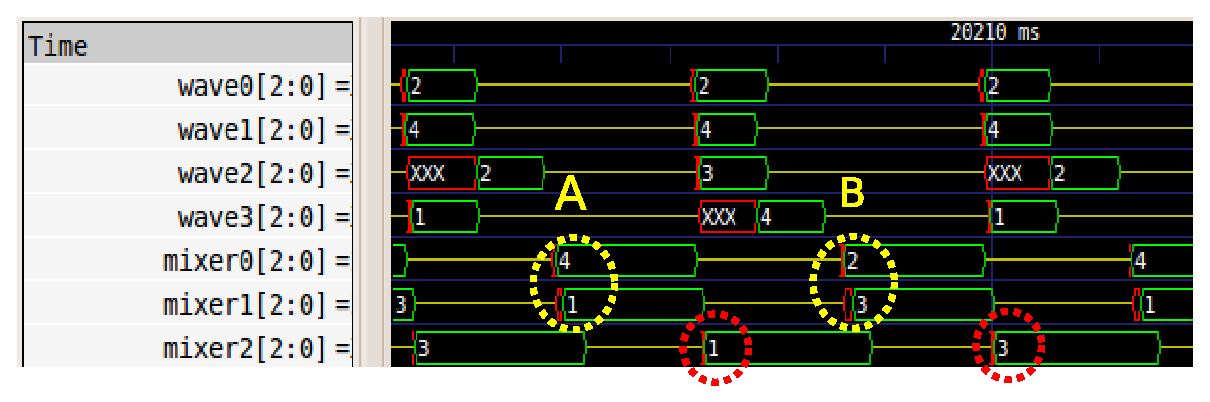
\includegraphics[width=\widefigure]{images/results_xeon/final_xeon.eps}
\caption{\figurecaption{trace TODO dire che sta a 32KB }}
\label{fig:trace_xeon}
\end{figure}

As we can see in Fig. \ref{fig:trace_xeon}, the scheduling performed is correct. We see that \textit{mixer2} can precede one of the waves and improve 
parallelism. We see that \textit{mixer0} chooses the best cpu in term of temporal locality, for example: in step A \textit{mixer0} chooses CPU4 and not 
CPU2, because on CPU2 was executed \textit{wave2}, therefore L1 cache could be dirty, instead on CPU4 the last task executed is \textit{wave1}, therefore 
L1 cache should be clean. Also in step B, it is possible to note how \textit{mixer0} take care about the last task executed on CPU4 choosing CPU2.

\begin{figure}[htbp]
\centering
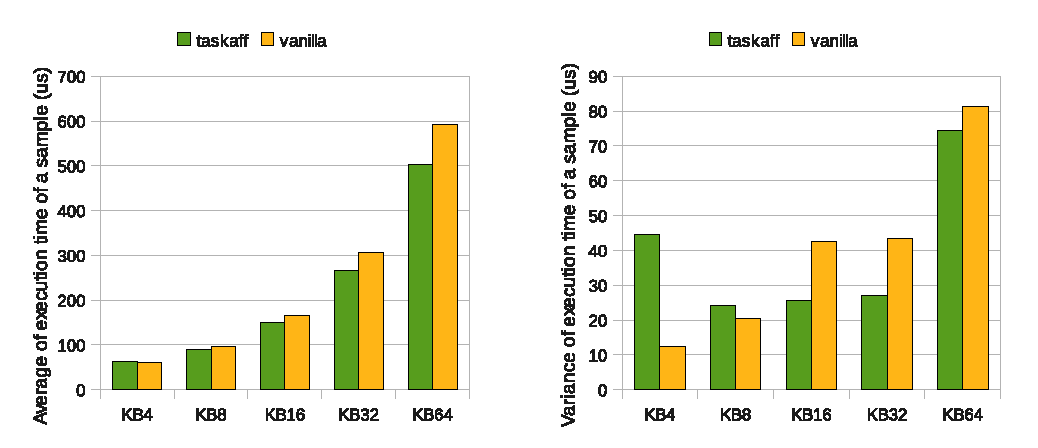
\includegraphics[width=\widefigure]{images/results_xeon/time_avg_var.eps}
\caption{\figurecaption{Average and Variance of execution time of a sample}}
\label{fig:time_avg_var_xeon}
\end{figure}

\begin{table}[htbp]
\begin{center}
\begin{tabular}{l|c|c|c}
	\hline
	& Speedup on Xeon \\ \hline
	& taskaff & vanilla \\ \hline
	$4KB$ & 2.45 (3.12) \% & 2.38 (1.82)\% \\ \hline
	$8KB$ & 2.47 (3.12) \% & 2.22 (1.83)\% \\ \hline
	$16KB$ & 2.47 (3.14) \% & 2.15 (1.87)\% \\ \hline
	$32KB$  & 2.51 (3.14) \% & 2.13 (1.9)\% \\ \hline
	$64KB$  & 2.52 (3.13) \% & 2.09 (1.92)\% \\ \hline
\end{tabular}
\label{tab:speedup_xeon_i7}
\caption{Speedup obtained with task-affinity and with vanilla on Xeon. Values in brackets represent ideal speedup}
\end{center}
\end{table}

\begin{figure}[htbp]
\centering
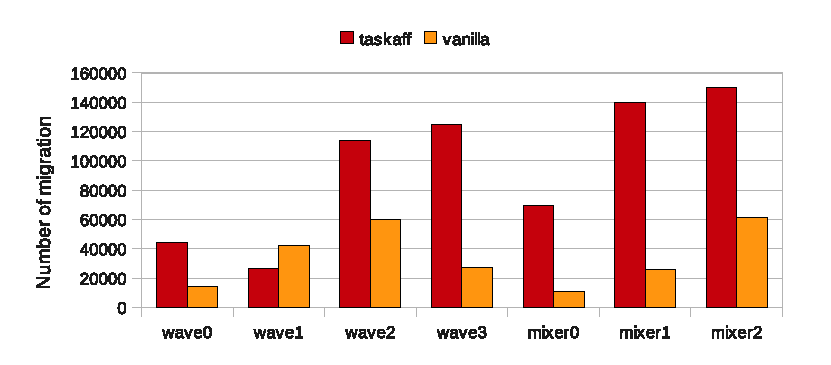
\includegraphics[width=\widefigure]{images/results_xeon/migration_xeon.eps}
\caption{\figurecaption{task migration on Xeon}}
\label{fig:migration_xeon}
\end{figure}

\begin{figure}[htbp]
\centering
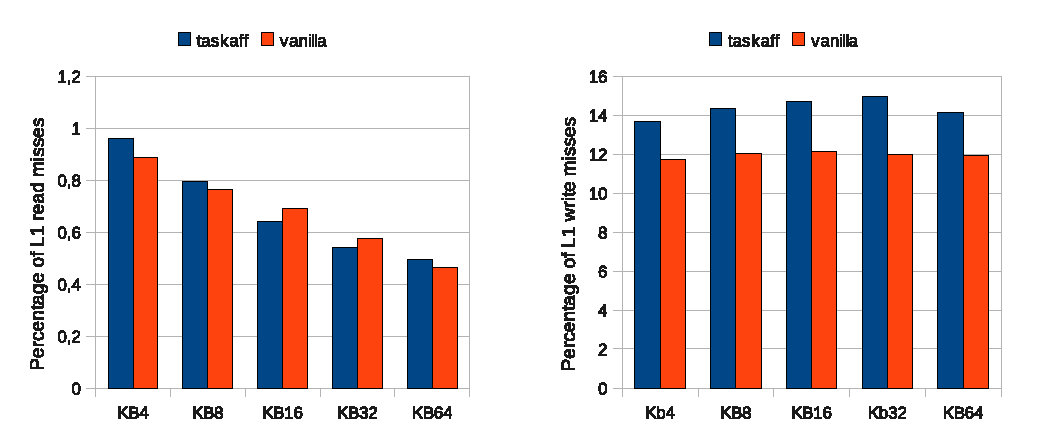
\includegraphics[width=\widefigure]{images/results_xeon/l1_load_store_xeon.eps}
\caption{\figurecaption{L1 Read and Write misses on Xeon}}
\label{fig:l1_load_store_xeon}
\end{figure}

\begin{figure}[htbp]
\centering
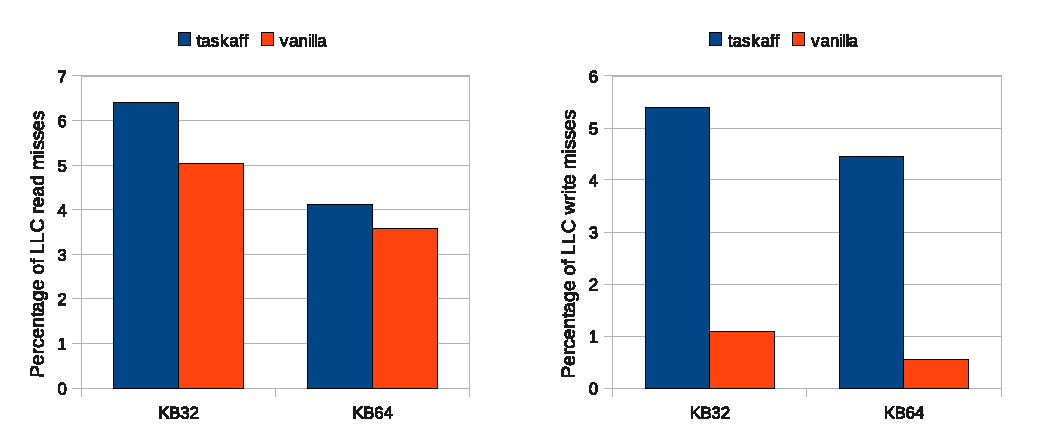
\includegraphics[width=\widefigure]{images/results_xeon/l2_load_store_xeon.eps}
\caption{\figurecaption{LLC Read and Write misses on Xeon}}
\label{fig:l2_load_store_xeon}
\end{figure}

%%%%%%%%%%%%%%%%%%%%%%%%%%%%%%%%%%%%%%%%%%%%%%%%%%%%%%%%%%%%%%%%%%%%%%%%%%%%%
\section{Intel i7}

\begin{figure}[htbp]
\centering
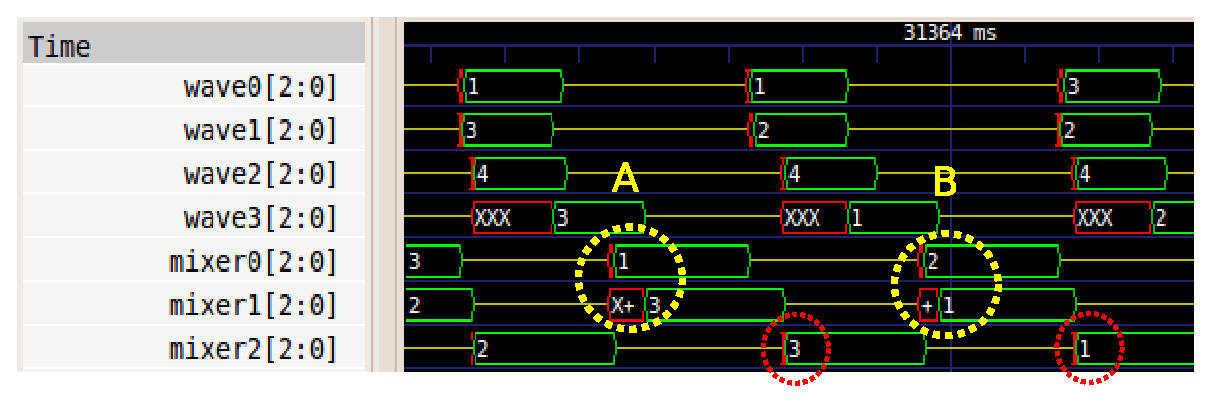
\includegraphics[width=\widefigure]{images/results_i7/final_i7.eps}
\caption{\figurecaption{trace TODO}}
\label{fig:trace_i7}
\end{figure}

Also in this case, Fig. \ref{fig:trace_i7}, the scheduling performed is correct. We can see how in step A and B mixers choose the correct CPUs according to
their task-affinity relationships.

\begin{figure}[htbp]
\centering
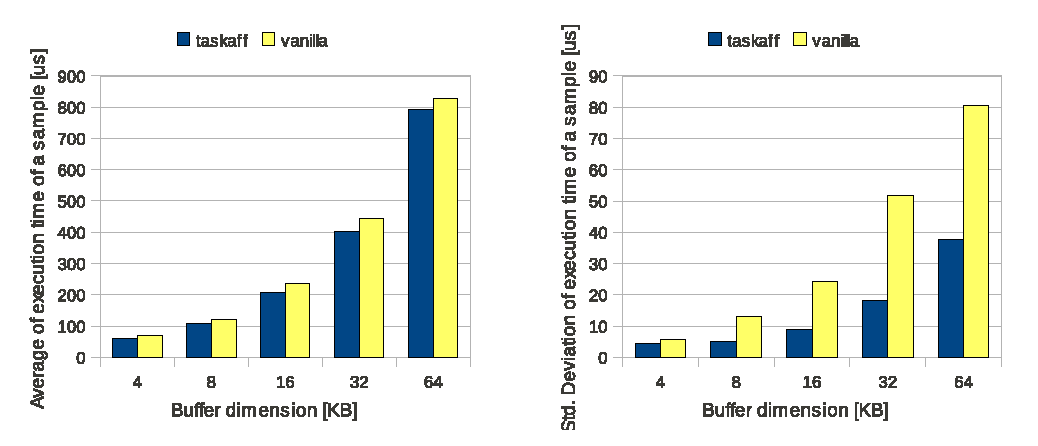
\includegraphics[width=\widefigure]{images/results_i7/time_avg_var_i7.eps}
\caption{\figurecaption{Average and Variance of execution time of a sample}}
\label{fig:time_avg_var_i7}
\end{figure}

\begin{table}[htbp]
\begin{center}
\begin{tabular}{l|c|c|c}
	\hline
	& Speedup on i7 \\ \hline
	& taskaff & vanilla \\ \hline
	$4KB$ & 2.56 (3.27) \% & 2.28 (2.09)\% \\ \hline
	$8KB$ & 2.6 (3.33) \% & 2.27 (2.11)\% \\ \hline
	$16KB$ & 2.6 (3.38) \% & 2.18 (2.13)\% \\ \hline
	$32KB$  & 2.63 (3.4) \% & 2.24 (2.15)\% \\ \hline
	$64KB$  & 2.65 (3.48) \% & 2.32 (2.16)\% \\ \hline
\end{tabular}
\caption{Speedup obtained with task-affinity and with vanilla on i7. Values in brackets represent ideal speedup}
\label{tab:speedup_i7}
\end{center}
\end{table}

\begin{figure}[htbp]
\centering
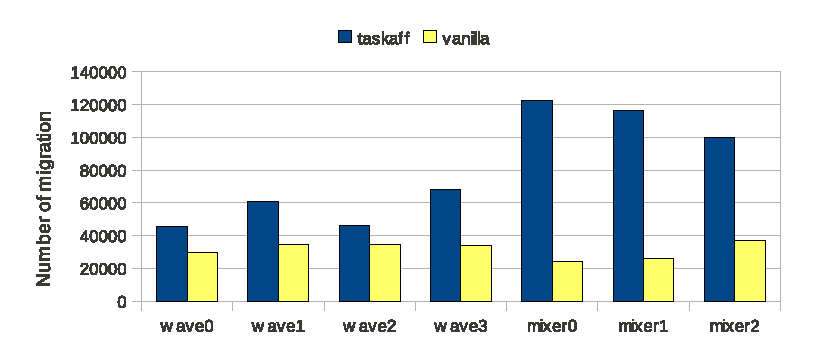
\includegraphics[width=\widefigure]{images/results_i7/migration_i7.eps}
\caption{\figurecaption{task migration on i7}}
\label{fig:migration_i7}
\end{figure}

\begin{figure}[htbp]
\centering
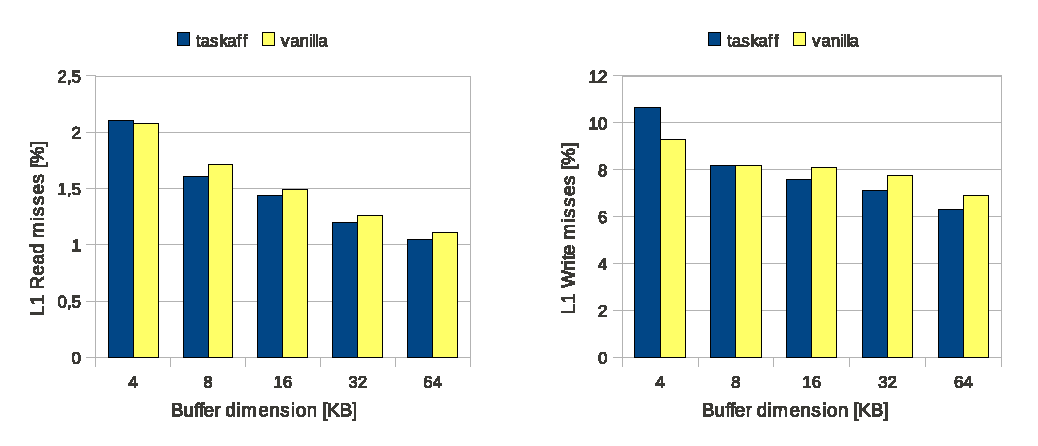
\includegraphics[width=\widefigure]{images/results_i7/l1_load_store_i7.eps}
\caption{\figurecaption{L1 Read and Write misses on i7}}
\label{fig:l1_load_store_i7}
\end{figure}

\begin{figure}[htbp]
\centering
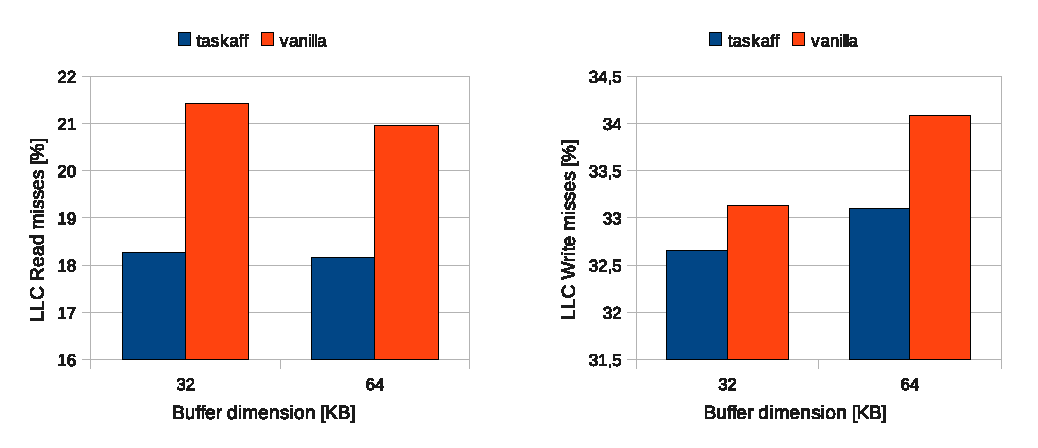
\includegraphics[width=\widefigure]{images/results_i7/l3_load_store_i7.eps}
\caption{\figurecaption{LLC Read and Write misses on i7}}
\label{fig:l2_load_store_i7}
\end{figure}

\newpage
%%%%%%%%%%%%%%%%%%%%%%%%%%%%%%%%%%%%%%%%%%%%%%%%%%%%%%%%%%%%%%%%%%%%%%%%%%%%%
\section{AMD}

\begin{figure}[htbp]
\centering
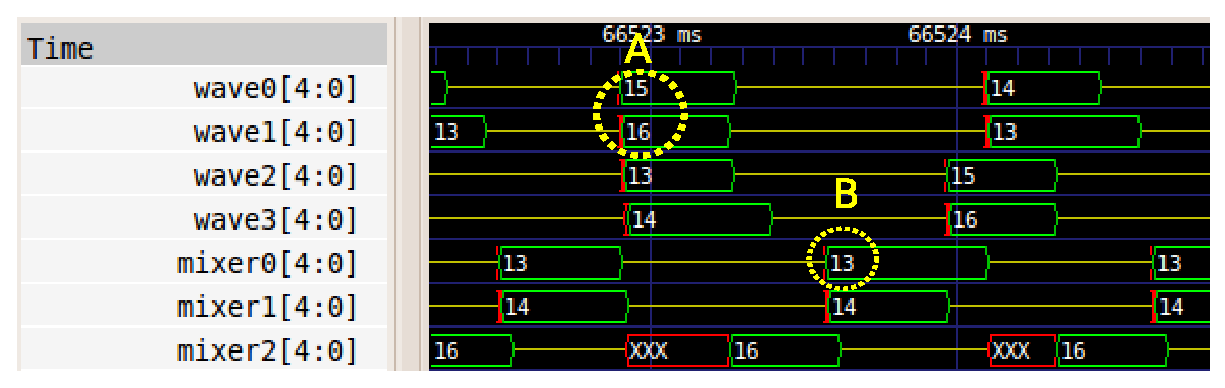
\includegraphics[width=\widefigure]{images/results_AMD/final_AMD.eps}
\caption{\figurecaption{trace TODO}}
\label{fig:trace_AMD}
\end{figure}

Unexplainably, task-affinity on this machine doesn't work. We can see in step B that \textit{mixer0} doesn't choose the correct CPU. AMD is a NUMA 
architecure and task-affinity patch it is developed for SMP architectures, therefore it could be necessary a revision of code in order to manage also 
NUMA architectures.

%%%%%%%%%%%%%%%%%%%%%%%%%%%%%%%%%%%%%%%%%%%%%%%%%%%%%%%%%%%%%%%%%%%%%%%%%%%%%
\section{Consideration on exeperimental results}

From previous graphics it is possbile to do some considerations:

\begin{description}

\item[throughput:] In both Intel Xeon and Intel i7, parallelism is improved. We can see in Fig \ref{fig:time_avg_var_xeon} an increment of throughput 
especially with 32 and 64KB, while at 4KB the increment is not very significant. This happens because, see in Fig. \ref{fig:4KB_xeon_results_van} 
\ref{fig:4KB_xeon_results_taskaff}, using buffer of 4KB, parallelism performed in vanilla is very similar to parallelism performed in task-affinity.

\begin{figure}[htbp]
\centering
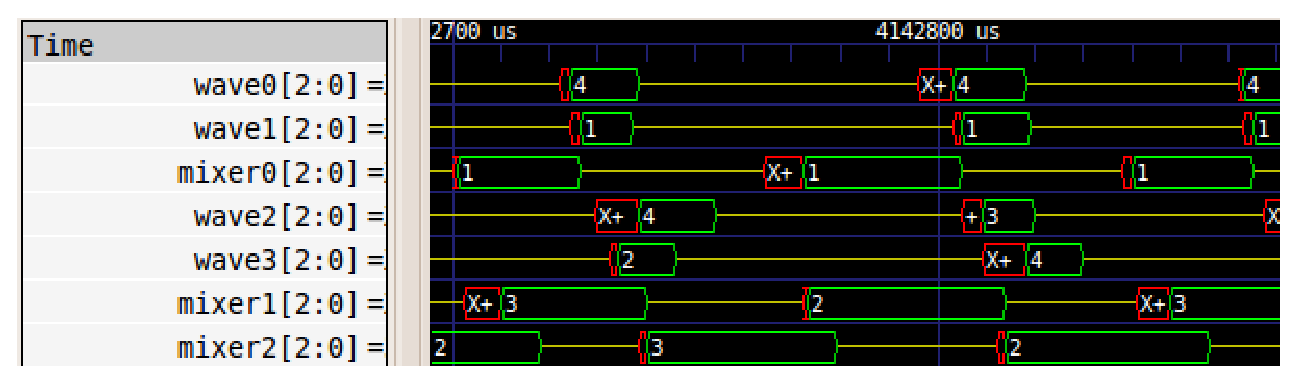
\includegraphics[width=\widefigure]{images/results_xeon/4KB_results_xeon_taskaff.eps}
\caption{\figurecaption{trace of benchmark execution on Xeon with buffer of 4KB using taskaffinity}}
\label{fig:4KB_xeon_results_taskaff}
\end{figure}

\begin{figure}[htbp]
\centering
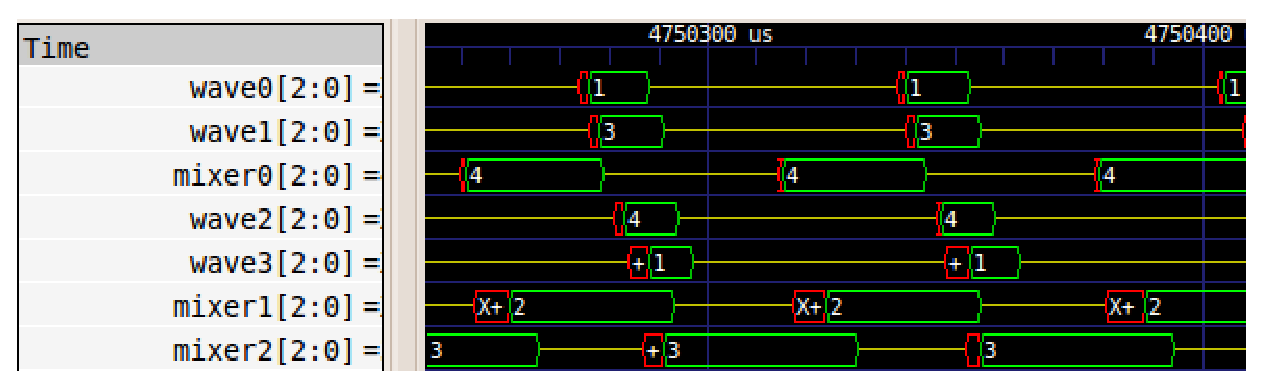
\includegraphics[width=\widefigure]{images/results_xeon/4KB_results_xeon_van.eps}
\caption{\figurecaption{trace of benchmark execution on i7 with buffer of 4KB using vanilla}}
\label{fig:4KB_xeon_results_van}
\end{figure}

As regard for speedups, we see that using task-afinity in both Xeon and i7, we have real speedups less than ideal speedups. This fact happens because the 
real performed scheduling is slightly different from ideal scheduling showed in Fig. TODO and real parallelism of the application is lower than ideal 
parallelism. Using vanilla, instead, real speedups are greater than ideal speedups, because real scheduling improve parallelism respect ideal scheduling, 
Fig. TODO. In fact if we see Fig TODO trace 4k we note that there is a fraction of \textit{mixer2} that is executed concurrently with others waves, while in
ideal scheduling \textit{mixer2} should be executed alone.

\item[migrations:] Number of migration is greatly increased, this is not due to architectural details or different buffer dimensions. This fact happens 
because, at each sample, \textit{mixer0} and \textit{mixer1} and waves are excuted on the same CPUs. Since in the next sample waves are waken up during the 
execution of \textit{mixer0} and \textit{mixer1}, they must be scheduled on CPUs different from which that have executed them in the previous sample. 
For this reason, at each sample, waves are executed on different CPUs and, consequently, also other tasks are executed on different CPUs at each sample.

\item[cache misses:] Because of worsening of L1 and LLC cache misses, Fig \ref{fig:l1_load_store_xeon} \ref{fig:l2_load_store_xeon}, on Intel Xeon 
predictability of the application is degradated Fig. \ref{fig:time_avg_var_xeon}, especially using small buffer dimension such as 4KB or 8KB. LLC miss rate 
is greatly increased in task-affinity, because, as explained in the previous chapter, a core can access to data that are in caches of its own die, 
therefore if a task migrates frequently between two different dies, at each migration it will have to warm up LLC cache and a cache miss will occur. The 
same goes for L1 cache misses, also in that case a migration between CPUs that are in different dies increase L1 miss rates. Nevertheless with dimension 
greater than 8KB and especially greater than 32KB predictability is improved. This means that miss rates on Intel Xeon doesn't influence significantly 
predictability of the application. On Intel i7, instead, thanks to inclusive shared LLC, a core can access to data contained in all caches of other cores, 
consequently, L1 and LLC cache misses are reduced. The diminishing of cache misses impacts significantly on application predictability 
Fig.\ref{fig:time_avg_var_i7}.

\item[migration functions:] As we can see from Fig. TODO graf in task-affinity \textit{pull\_rt\_tasks} executes more work than in vanilla. 

TODO snippet pull per l\'if e per il ciclo sotto

The explanation is simple: at the line TODO in Fig. snipp there is a check for overloading runqueues. If in the system there is any overloading runqueue, 
\textit{pull\_rt\_tasks} searches which runqueues are overloaded and try to pull task from them. With task-affinity, only 3 waves are executed concurrently 
and one wave has to wait that \textit{mixer2} finish, therefore at each sample there is an overloaded runqueue in the system. For this reason, when 
\textit{pull\_rt\_tasks} is called, almost certainly it will enter in loop in order to pull tasks from overloaded runqueue. With vanilla instead, all waves 
are executed concurrently, therefore there are less probabilities to have overloaded runqueues. It is interesting to note that number of call of 
\textit{pull\_rt\_tasks} is equal in both task-affinity and vanilla, because \textit{pull\_rt\_tasks} is called at each context-switch, but obviously, in 
vanilla \textit{pull\_rt\_tasks} will exit at line TODO snip. Overhead of \textit{pull\_rt\_tasks} influences predictability of application especially with
buffer of 4KB because execution time of each thread is relatively small.

\end{description}


